\chapter{Introduction}
In this Chapter the RISC-V and V-Extension concepts relevant for this thesis are presented and discussed together with  the verification notions.
Furthermore, an overview on the context of this project is given,  explaining the Vector Processing Unit (VPU) implemented and then showing the Universal Verification Methodologies (UVM) adopted.

Firstly, the RISC-V Instruction Set Architecture (ISA) is briefly illustrated, proceeding with an overview on all the major extensions provided by the \mbox{RISC-V} foundation. The Concepts section is then closed with some knowledge about the Verification process and its main tools. 

Finally the theory is contextualized by the implemented VPU and on the used UVM structure. Those allow to better understand the contributions done in this thesis, contributions that are then explained into the next Chapter.






\section{Concepts}
\subsection{RISC-V}
RISC-V is an open, extensible and free ISA. It was initially only designed to support computer architecture research and education~\cite{RISC-V-Instruction-Set-Manual}.
The project, began at the Berkeley University of California in 2010, published the first ISA User Manual in 2011. 

The RISC-V ISA is implemented as a base integer ISA, but it is modular and so supports many instruction encodings.
This ISA is provided under open source licenses, and it is gaining a lot of popularity due to its open nature. 
Mainly there are two primary base integer variants, RV32I and RV64I, which provide 32-bit or 64-bit user-level address spaces respectively.

\subsubsection{Extensions}

RISC-V is designed to have a good customization which is the reason why it is provided with the possibility to be extended, but the base integer instructions cannot be redefined.
There are two kinds of extensions:
\textit{standard} and \textit{non-standard}.
\begin{itemize}
    \item The \textit{standard} ones need to be compatible with all the other standards and they should also aim to be generally useful.
    \item The \textit{non-standard} ones can be highly specialized in some task and therefore they may conflict with other extensions.
\end{itemize}

For general development, as defined in the specification document~\cite{RISC-V-Instruction-Set-Manual}, some of the standard extensions are predefined:
\begin{itemize}
    \item "\textbf{I}" is the base integer extension and contains integer computational instructions, integer loads, integer stores, and control-flow instructions. It is mandatory for all RISC-V implementations.
    
    \item "\textbf{M}" is the standard integer multiplication and division extension, it allows to multiply and divide the values held in the integer registers.
    
    \item "\textbf{A}" is the standard atomic instruction extension. It is useful to have atomic instructions for inter-processor synchronization. In fact, with this extension is possible to read, modify, and write memory atomically. 
    
    \item "\textbf{F}" is the standard single-precision floating-point extension. It adds floating-point registers, single-precision computational instructions, and single-precision loads and stores. 
    
    \item "\textbf{D}" is the standard double-precision floating-point extension. Advantageous when the F extension is not enough, it expands the extension and adds double-precision computational instructions, loads, and stores.
    
    \item "\textbf{G}" is the denotation for an integer base plus these four standard extensions (“IMAFD”).
    
    \item "\textbf{V}" is the standard Vector Extension. It is designed to add the possibility to perform vector operations, allowing performance and efficiency. The thesis will focus only on this extension.
\end{itemize}


The design philosophy of the RISC-V projects is based on modularity: the base ISA will not change over time, but new extensions will be available and new feature will be added. Which is a major feature because of the difficulty in finding general useful extension beyond the ones already existing. Therefore, it would not be convenient to constantly add new features to the base ISA and then have to keep track of that at a later time.


\subsubsection{Base instructions}
In Figure \ref{riscv-base-instruction-formats} it is possible to see how the base instruction are composed.

\begin{figure}[H]
    \centering
    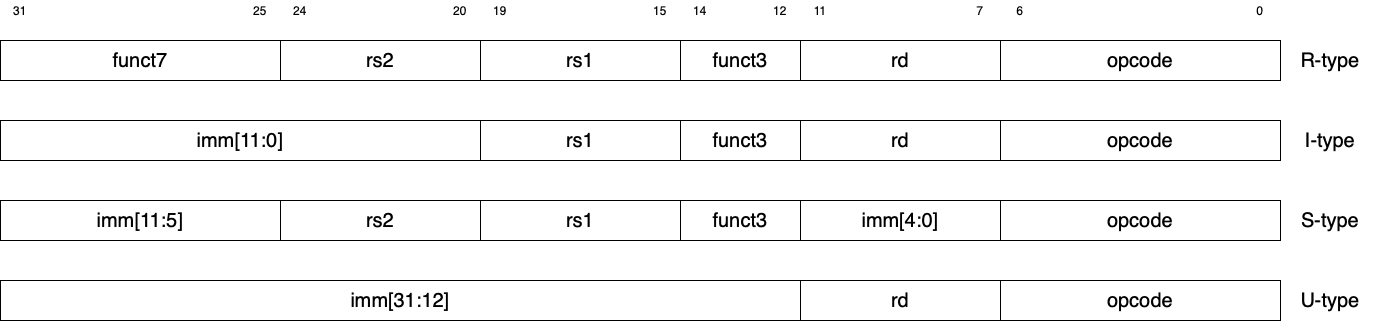
\includegraphics[scale = 0.27]{Chapter_1/img/riscv-base-instruction-formats.png}
    \caption{RISC-V base instruction formats. \cite{RISC-V-Instruction-Set-Manual}}
    \label{riscv-base-instruction-formats}
\end{figure}

It is important to notice that RISC-V is a load-store architecture, which means that only load and store operations can have access to the memory.
It is a very convenient organization, because it reduces the average time-per-operation and guarantees a good functioning of the pipelined structure.

The instruction also supports signed byte and half word loads, which is very advantageous when working with signed byte and half word data types.

In Figure \ref{riscv-load-store} it is possible to see how the load-store instructions are composed, and that the LOAD is an I-type op and the STORE is an S-type op.

\begin{figure}[H]
    \centering
    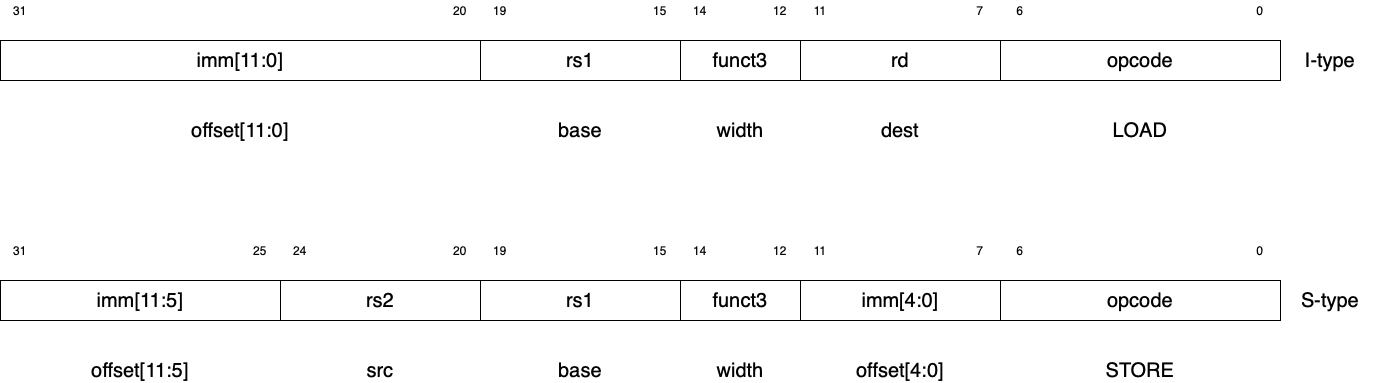
\includegraphics[scale = 0.27]{Chapter_1/img/riscv-load-store.png}
    \caption{RISC-V load/store instruction formats. \cite{RISC-V-Instruction-Set-Manual}}
    \label{riscv-load-store}
\end{figure}


\subsection{Parallelism, Vectors and the V-Extension}
During the last years, the parallel architecture is gaining inertia on the processors field. This is happening because the real world has parallel behaviour and so the hardware we use to compute simulations and calculus needs to be likewise~\cite{Parallel-Computing}.

%But why this is happening now and not before?\\
%In the past, parallel computing efforts have shown promise and gathered investment, but uniprocessor computing did always eventually prevailed, what is different now?\\
Also, most of the paradigms that led to the decision of using a single core, are now changing quickly as the technology changes its needs.
In fact, as the technology scales down to the nanometers, the power and the energy consumptions are becoming a problem. Also, the cost of a single transistor is significantly lower.

%However the multicore solution does not still meet the conformity for old binaries compilations and it could be difficult to program. Thus, the solution of a parallel architecture with "manycores" seems to be the right one.\\

A solution to the efficiency problem are the VPU (Vector Processing Units) working with single instruction multiple data (SIMD), in this way it possible to maintain the binaries easy to program, but very powerful in term of data computation..

A famous example of a vector architecture is the Cray-1, presented in 1975.
The Cray-1, a load/store architecture, was designed for Supercomputing and its major feature was to have a scalar mode along the vector one. This was advantageous because high performances are not always useful.

\subsubsection{Time efficiency}
As shown in Figure \ref{Multithreading}, with standard multithreading there will often be some empty thread along with the running ones, causing a loss in the efficiency.
\begin{figure}[H]
    \centering
    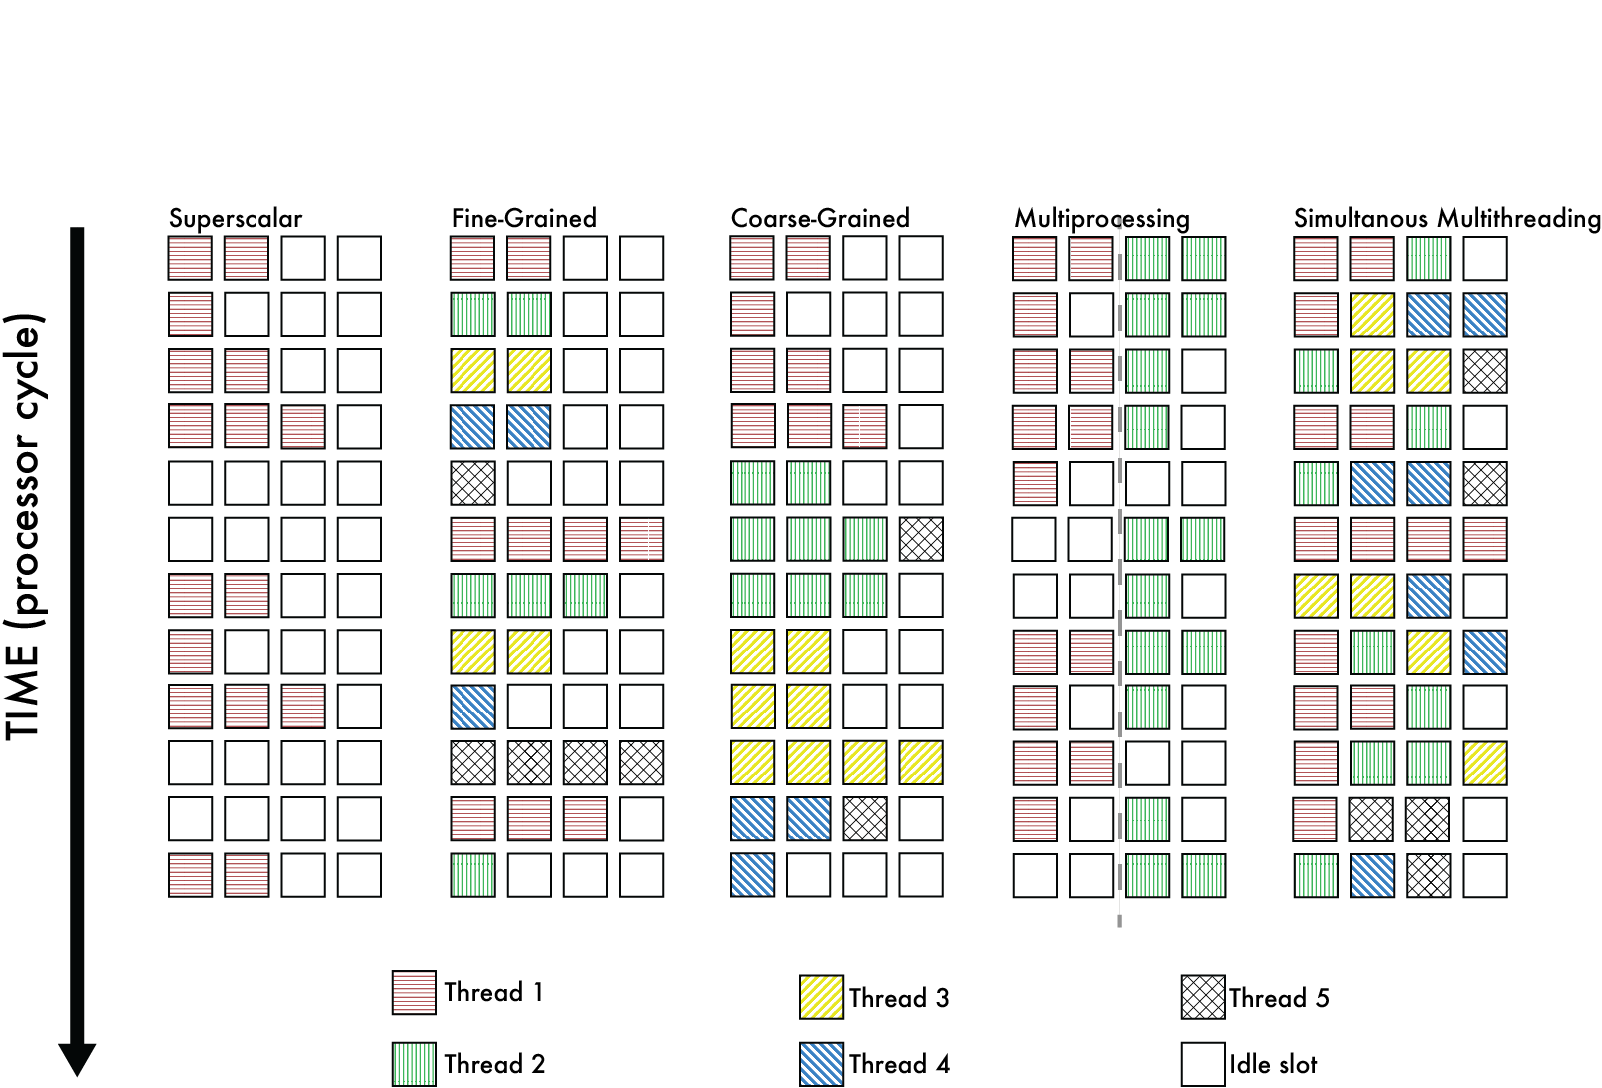
\includegraphics[scale = 0.5]{Chapter_1/img/threads.png}
    \caption{Multithreading Processor Clock Time usage  \cite{L15-Krste}}
    \label{Multithreading}
\end{figure}

Indeed the major advantage with the vector computation is the condensation of the processor usage. 
So that the usage will not be distributed as for standard multithreading processors, but it will have full usage for some cycles and none usage for others~\cite{L15-Krste}.

\begin{figure}[H]
    \centering
    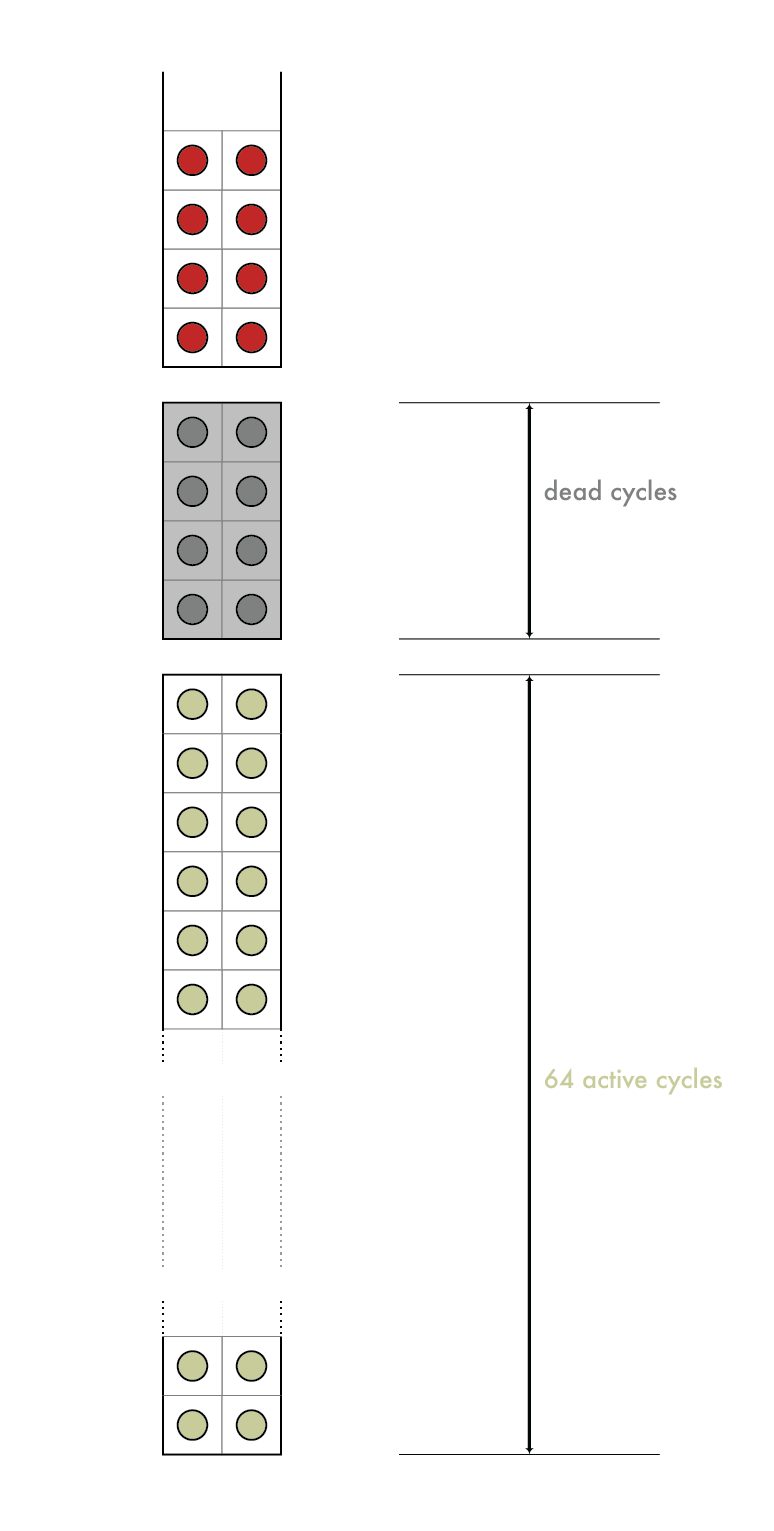
\includegraphics[scale = 0.4]{Chapter_1/img/time-usage.png}
    \caption{Vector Processor Processor Time usage \cite{L15-Krste}}
    \label{Vectoring}
\end{figure}

It is shown in Figure \ref{Vectoring} how the processor usage is condensed in some cycles and then empty for others. That happens because the vector operations need some clock cycles to start up. So based on the length of the pipeline, there will be some dead cycles.
This means the latency increases, because each operation adds some dead cycles that need to be waited before a new operation can start.

But, this drawback can be used to increase the efficiency with modern low-power techniques. In fact, it was shown~\cite{Lemuet2006} that the Vector Accelerators, while \emph{improving performances up to 10X}, can also \emph{improve energy efficiency of \mbox{40-50\%} on loop kernels and \mbox{10-20\%} on larger program segments}.
In Figure \ref{Vector-Latency} it is possible to see how a vector needs to wait the previous one to be completed before starting, and so why the latency increases. 

\begin{figure}[H]
    \centering
    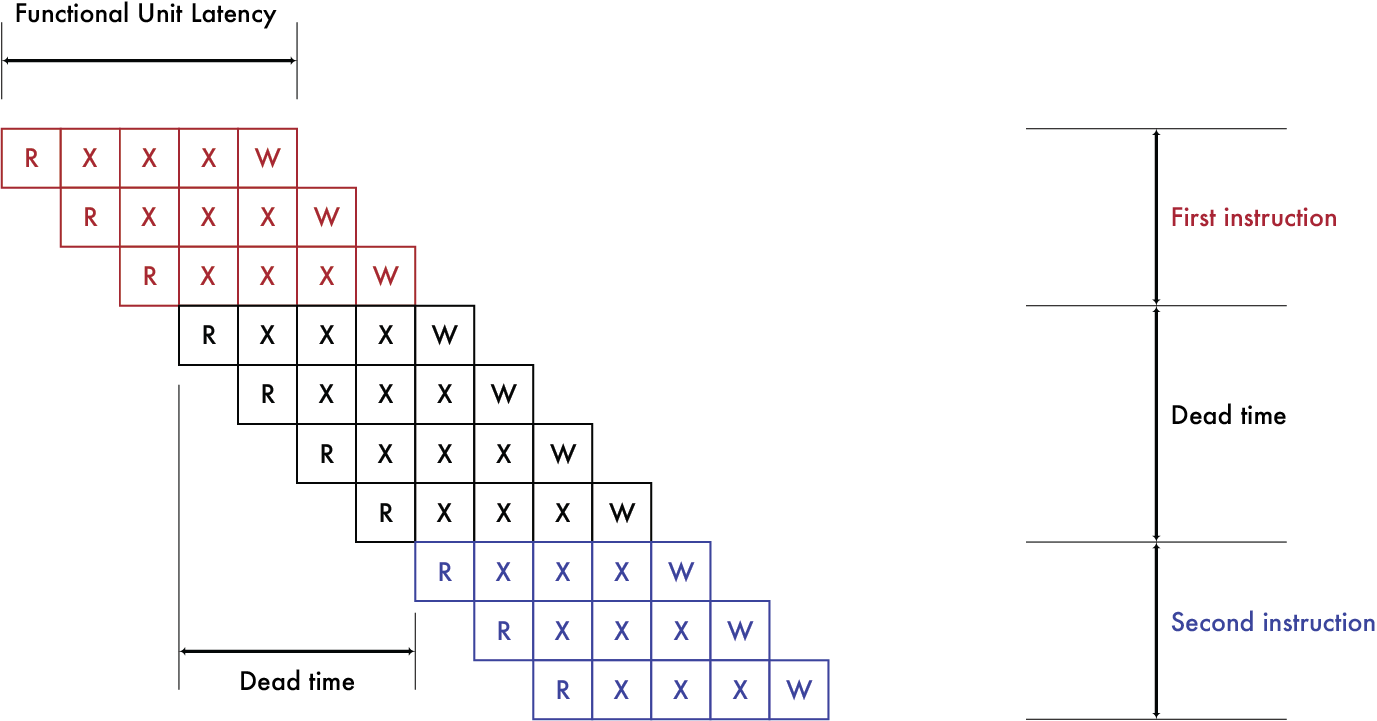
\includegraphics[scale = 0.5]{Chapter_1/img/lat-pen.png}
    \caption{Latency penalty on vector processing units \cite{L15-Krste}}
    \label{Vector-Latency}
\end{figure}


The design implementation that is been used for the EPI project and so in this thesis is the V-Extension (V stands for Vector), and it is in current development. The reference is the V-Extension 0.7.1.

The vector extension adds 32 vector registers, and 5 unprivileged CSRs (\emph{vstart}, \emph{vxsat}, \emph{vxrm}, \emph{vtype}, \emph{vl}) to the base scalar \mbox{RISC-V} ISA\cite{riscv-v-specs}.
There are also 8 vector predicate registers (vp0-vp7). The CSRs vectors define the configurations.

\begin{table}[H]
    \centering
    \begin{tabular}{|l|l|l|l|}
        \hline
        \llgray Privilege & \llgray Name   & \llgray Description               \\ \hline
        URW       & vstart & Vector start position     \\ \hline
        URW       & vxsat  & Fixed-point Saturate Flag \\ \hline
        URW       & vxrm   & Fixed-Point Rounding Mode \\ \hline
        URO       & vl     & Vector length             \\ \hline
        URO       & vtype  & Vector data type register \\ \hline
    \end{tabular}
    \caption{RISC-V's CSRs}
    \label{CSRs}
\end{table}

The datatypes and operations supported by the V-extension change based on the
base scalar ISA~\cite{riscv-v-specs}.\\


The vector unit must be configured before being used. 
I.e. the active vector length is held in the CSR \emph{vl}, which can only hold values between 0 and MVL (Maximum Vector Lenght parameter) inclusive.
The active vector length is usually written with the \textbf{\emph{setvl}} instruction.

\subsubsection{Vector instructions}
Beside the base instructions that we can expect from a Vector Architecture (such as a move, add, xor and so on) it is also possible to find some useful operations related to the nature of the vector calculus~\cite{riscv-v-specs}:
\begin{itemize}
    \item \textbf{vectorial load/store}: are used to copy data between vector registers and memory. These instructions can be strided or indexed. The strided ones index the vector elements referring to a starting element and then adding (or subtracting) a certain stride to the base address. This kind of load/store is very fast, in particular in some special cases (as unit-strided or some optimized power of 2).
    
    The vector elements into the indexed ones are basically pointed with a vector of indexes, added to a base address. This process does really slows down the operation but allows to directly select the elements.
    
    \item \textbf{widening/narrowing}: these operation are used to increase or decrease the size of the vector's contents. In fact, they are very useful when performing operations that need to increase the result size (as example a multiplication between to integer at 32 bit needs to have 64 bit to not loose information). There are also few operations that require the inverse resizing, as for the narrowing.
    
    \item \textbf{rgather}: those are very particular operations which are very advantageous when manipulating vectors. They allow to index a vector using another vector as index. Therefore, various patterns are possible. The pseudo code representing this operation is the following: 
    \begin{lstlisting}[language=Verilog,style=verilog-style, numbers=none]
  for (i=0; i<N; ++i)
    x[i] = y[idx[i]];
    \end{lstlisting}
    where \emph{y} is the starting vector, \emph{idx} is the index vector and \emph{x} is the result vector.
    
    \item \textbf{reduction}: finally, the reduction can perform an operation between a scalar and a vector and give a scalar as result (an easy example could be to calculate the maximum value between all the value contained in a vector and one scalar, the result would either be one of the element of the vector or the scalar).
    
\end{itemize}


Finally, all those operations can be \textit{masked}. The masking is a common operation when there is branching or when complex patterns emerge.
Normally one bit of the mask represent a whole word or byte into the vector. This bit indicates if the operation of the instruction should be performed for that specific element of the vector.

\subsection{Verification}
As the technology scales down, conflicting requirements for high performance, low-power and area arise. 
This lead to a complex design and to elevate the costs.

It is possible to see in Figure \ref{verification-tecnology} how the cost for verification increases drastically with the shrinking of the technology node.


\begin{figure}[H]
    \centering
    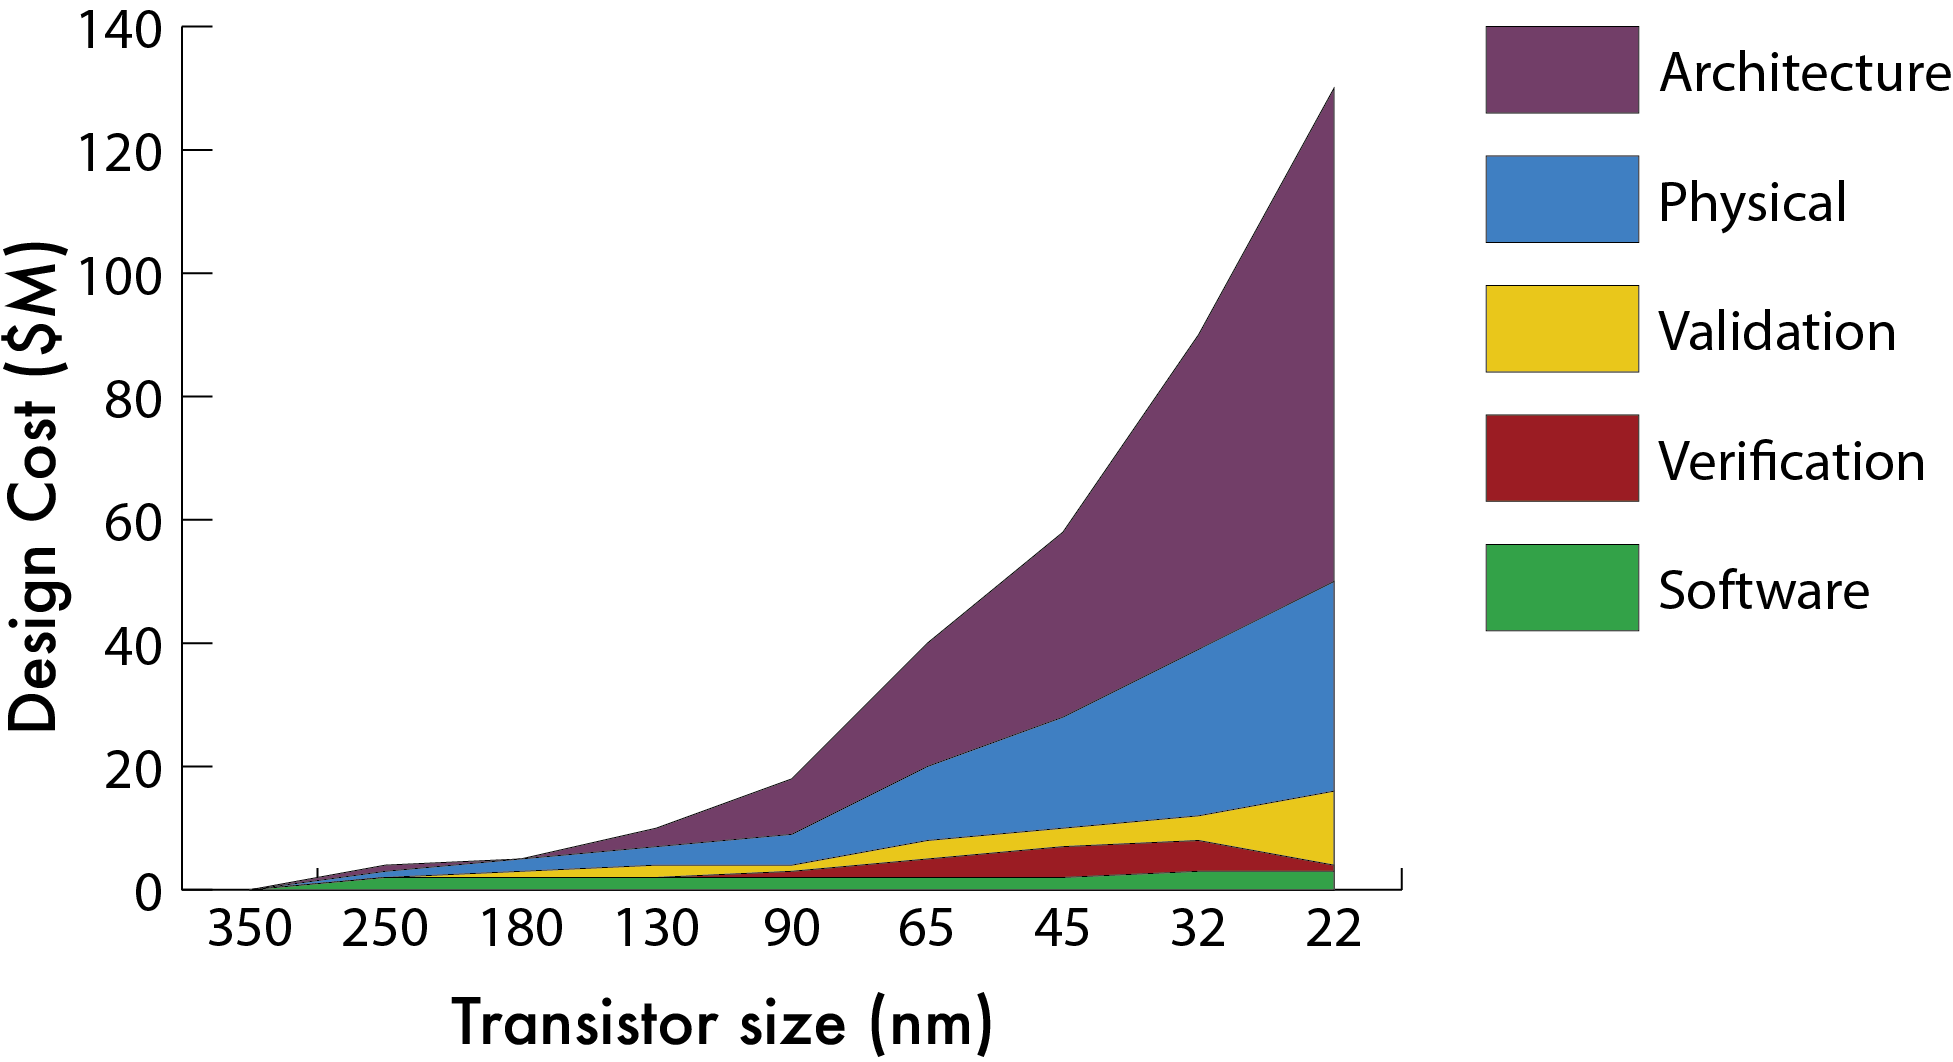
\includegraphics[scale = 0.4]{Chapter_1/img/cost-scale.png}
    \caption{The design cost vs the technology node \cite{verification-book-2018}}
    \label{verification-tecnology}
\end{figure}

Verification is responsible to make sure that the design is in track with the specification. So, if the design complexity increases, the same does its verification process.

This is of course an issue for the time-to-market. 
In particular functional design verification takes \mbox{40–50\%} of the project resources. In other words, increasing the productivity of functional design verification and shorten the design / simulate / debug / cover loop is an essential task \cite{verification-book-2018}.

Moreover, the compounded complexity grows faster then the compounded productivity. This gap only means the verification needs to be faster and hence needs to implement more techniques.
It is possible to see a study on the complexity/productivity gap in Figure \ref{complexity-gap}
\begin{figure}[H]
    \centering
    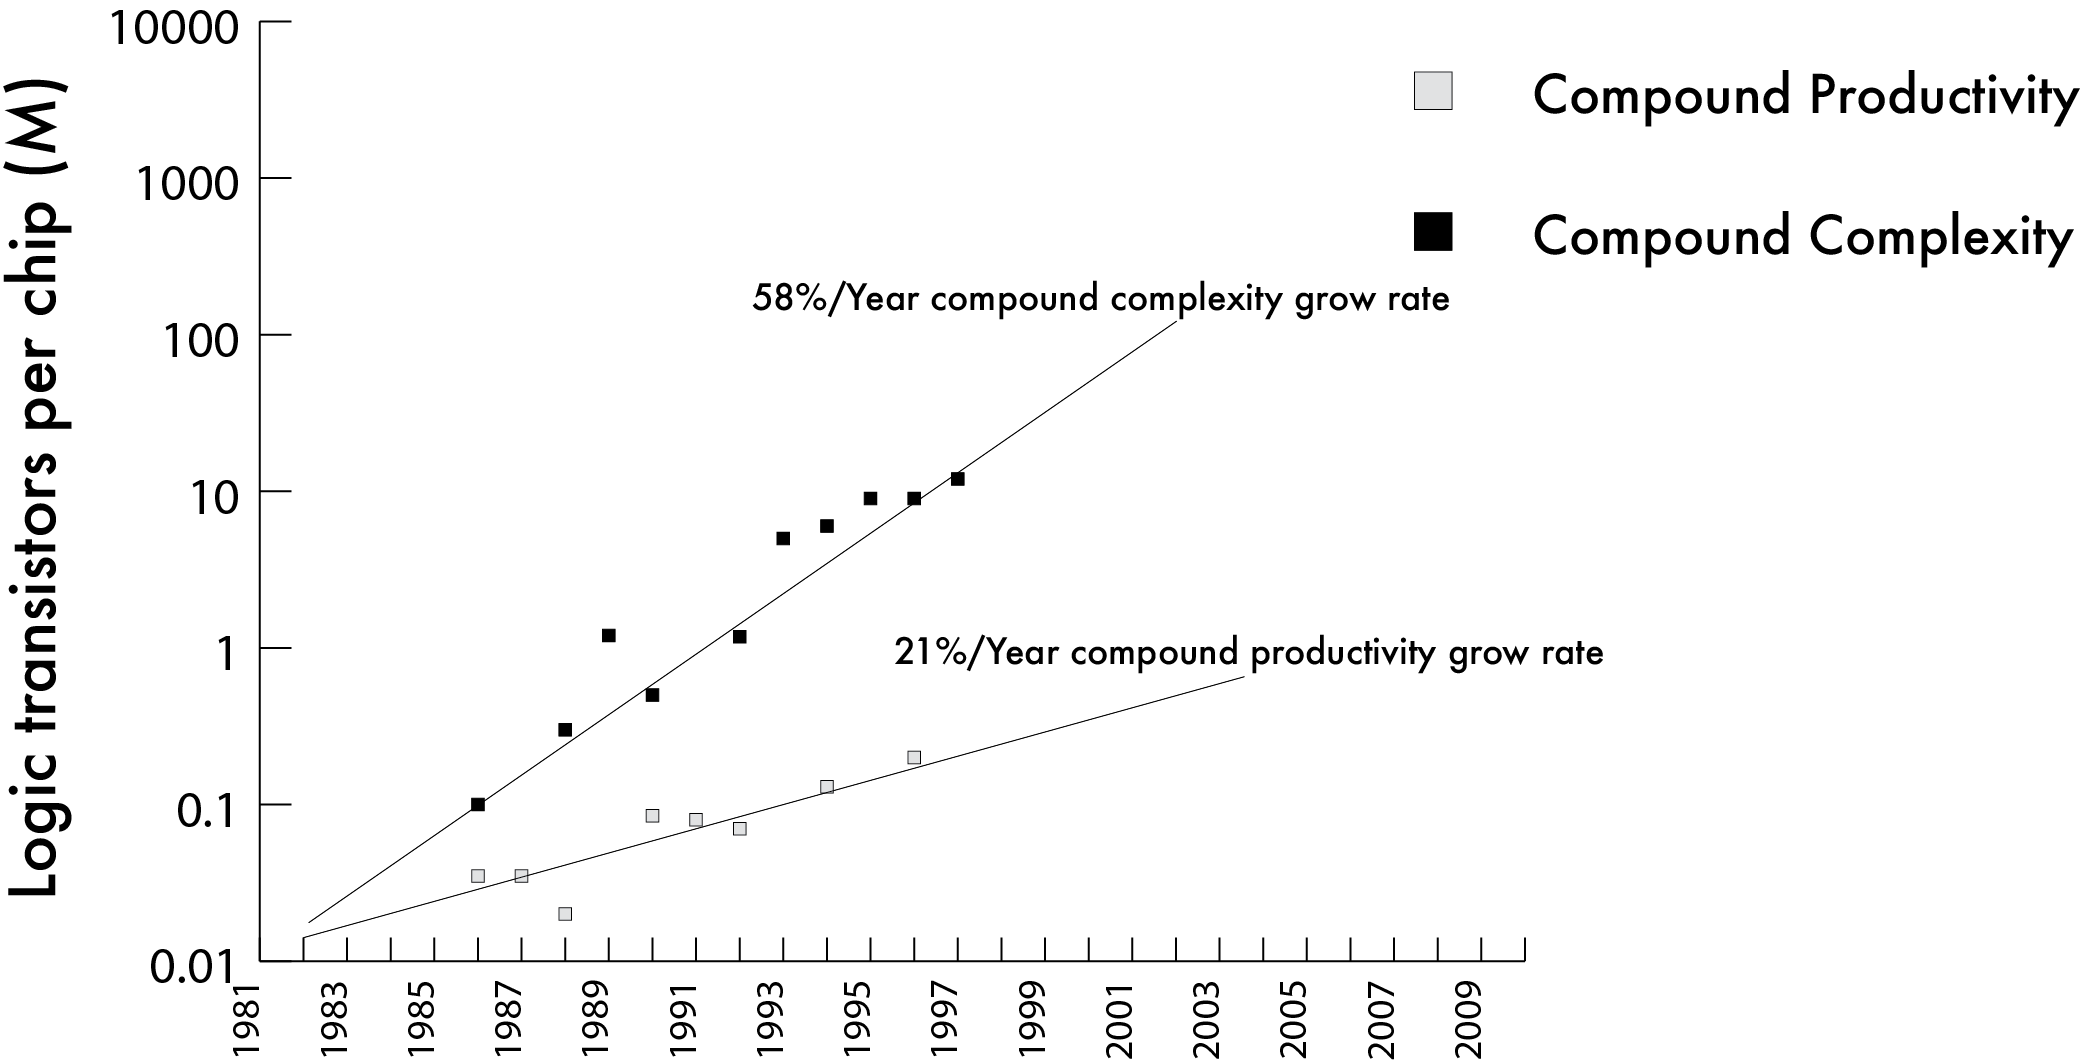
\includegraphics[scale = 0.4]{Chapter_1/img/prod-compl.png}
    \caption{The gap between the complexity and the productivity \cite{verification-book-2018}}
    \label{complexity-gap}
\end{figure}

This graph shows how the complexity rate is higher than the productivity rate during the years. This means that it is not possible to reach an equity only by increasing the number of tests or by adding some more checkers. More advanced techniques are needed to cope with the growing complexity.

In order to verify an RTL design, its specifications need to be stated as code. In this thesis all the tools implemented for the verification process are wrote in \emph{SystemVerilog}. 
SystemVerilog is an hardware description language, born as an evolution of the Verilog language. Some extensions such as Objective-Oriented Programming elements and specific keywords for verification tools were added to it. The functionalities of a design can be stated by using the \textbf{\emph{checkers}}.

\subsubsection{Checkers}
They are mainly composed by \emph{assertions} and \emph{assumptions}, some really powerful statements used to define the constraints of the DUT’s behaviour.

Assertions and assumptions are syntactically identical, but the first one refers to the output signals while the second one to the input signals.
They are mainly composed by two parts which are both conditions, even though they act differently. The first part is a condition to \textit{"fire"}, this means that when the condition is true the assertion, or assumption, starts checking for the second part.\cite{verification-book-2016}

The second part is another check on some condition, and can reveal the result of the check. At this point the possible results are \textit{True} or \textit{False}.

Both of them can be time consuming, and conditions on the edge are possible.
It is also possible to create \textit{properties} and \textit{sequences} and then embed them into the assertions, in this way it is possible to reuse those parts.

Let's now see the basic structure of an assertion.
\bigskip

\linespread{1}
\begin{lstlisting}[language=Verilog,style=verilog-style, backgroundcolor=\color{lyel_palette}, frame=tlb]
property property_1;
    @(posedge clk_i)
	a |-> b;
endproperty : property_1

assertion_1 : assert property ( disable_iff(rst) property_1) else $error("")

\end{lstlisting}
\linespread{1.2}
\bigskip

Basically if \emph{a} is HIGH('1') then \emph{b} is also expected to be HIGH('1').

The functionality is expressed into the property, then it is asserted into the assertion. It could be possible to recall tasks or processes, in this way it is possible to have more computational capabilities.
It can also provide an error message to better identify the problem during simulations.
When the signals into the \emph{disable\+iff} function are asserted (in the example above it is the \emph{rst} signal) the assertion is disabled. This means that the assertion does now need to be re-fired with a new starting condition.


\subsubsection{Functional verification}
The functional verification needs to verify whether the functionalities described into the specifications are met into the design. In order to verify functionally, the functionalities need to be defined. This is a very important part of the process, as this translation is never perfect and often highlights some critical points into the specs, such as omissions or inaccuracies. The functional verification is performed using simulations, this means that time is required to simulate the design behaviour and to check it against its specifications.

In functional verification the assertions and the assumptions are implemented in the simulation process to verify to correctness of the RTL design.

In Figure %figura TODO
it is possible to visualize how assertions and assumptions are used to verify functionally the RTL design.

\subsubsection{Formal verification}
The formal verification can be done in different ways: \textit{theorem proving}, that tries to prove the equivalence between specifications and design by using mathematical reasoning; \textit{equivalence checking}, useful when performing optimization to the design, trying to demonstrate that the various versions are mathematically equivalent; and \textit{model checking}, which try to find counter example on the behaviour of the design, and, if a counterexample exists, the Formal tool provides an example of the specific case to demonstrate the falsity. It is performed using \emph{assumptions} to assume the design behaviour and then using \emph{assertions} to test it.


As already mentioned, the assertions and the assumptions in simulations are treated equally . This is not true in the formal verification.

The aim of formal verification is to mathematically prove properties of a system, usually at design time~\cite{verification-book-2018-formal}.
The formal tool, in this project, was only used to perform model checking.

In order to be performed, the formal assertions verification only needs to instantiate the RTL file and the checkers file. Then it uses the assumptions as drivers for the RTL, and finally it tries to prove wrong the assertions using mathematical simplifications.

Hence, here it is possible to see how the assumptions work differently. If a property is assumed it can never be proved wrong. Only assertions need to be checked.

The tool used is provided by Mentor, and it is called Questa Propcheck.
There are different possible outcomes occurring while verifying:
\begin{itemize}
    \item \textbf{proof}: starting at the initial state, no legal stimulus exists that causes in the assertion to be violated. It is normally proven in the first 10-100 cycles;
    
    \item \textbf{firing}: a counterexample to the assertion exist, this means that there is a bug in design, or the specifications are not well defined;
    
    \item \textbf{firing with warnings}: a counterexample to the assertion exist, but it does not use primary inputs. This means that there are uncontrolled internal values that cause a fail;
    
    \item \textbf{inconclusive}: the formal analysis timed out before demonstrating the assertion. This could be also meaning the complexity is too high to be elaborated with math tools; 
    
    \item \textbf{bounded proof}: a proof exists to the assertion but only to a certain depth;
    
    \item \textbf{vacuous proof}: the case is vacuously proven when the assertion is always true given the assumptions. This means probably there is some mistake into the assumptions or the assertions.
\end{itemize}

In Figure %figure complexity/time TODO
are graphically summarized all the possible outcomes previously exposed.





\subsubsection{Coverage}
The whole process of verification does also need to have a direction. Coverage is employed to do it.

Coverage is very useful and can be performed on functionalities or code:
\begin{itemize}
    \item functionality: it measures the cover of all the functionalities stated by the specifications. This approach makes it possible to assure that all the requirements are met. But this also means that there is no information about unused RTL.
    
    \item code: it measures the cover of the RTL code. This means that it is possible to acknowledge whether there is unused logic and possibly some branch of the flow. Although, this implies that there is no check about the functionalities implemented.

\end{itemize}

The main goal is to take the coverage to 100\%. But at the same time it is easy to fool the coverage, because it depends on how the cases are taken into account.

In order to use all of these techniques there is the need of a structure to contain and control them.
This structure is designed following the \textbf{\emph{Universal Verification Methodology}} (UVM). The UVM is thought to verify circuits designs, and it is provided of Object-Oriented Programming elements, in order to enhance reusability. Later on this Chapter the particular case of this work is discussed.

\section{Context}
Prior to start, it is important to highlight that the VPU is designed to be the co-processor of a scalar core named Avispado. This core is under development by SemiDynamics, which works together with the BSC at the EPI project. In order to implement and test the VPU a simulator of the Avispado core was used, it is called Spike. It was initially developed to simulate RISC-V core, but for this project it was extended to simulate also the Vector-Extension. So, Spike is simulating both the core and the VPU, to use it as a scoreboard.
In Figure \ref{avi-vpu} it is possible to see the interface between Avispado and the VPU for all the instructions.

\begin{figure}[H]
    \centering
    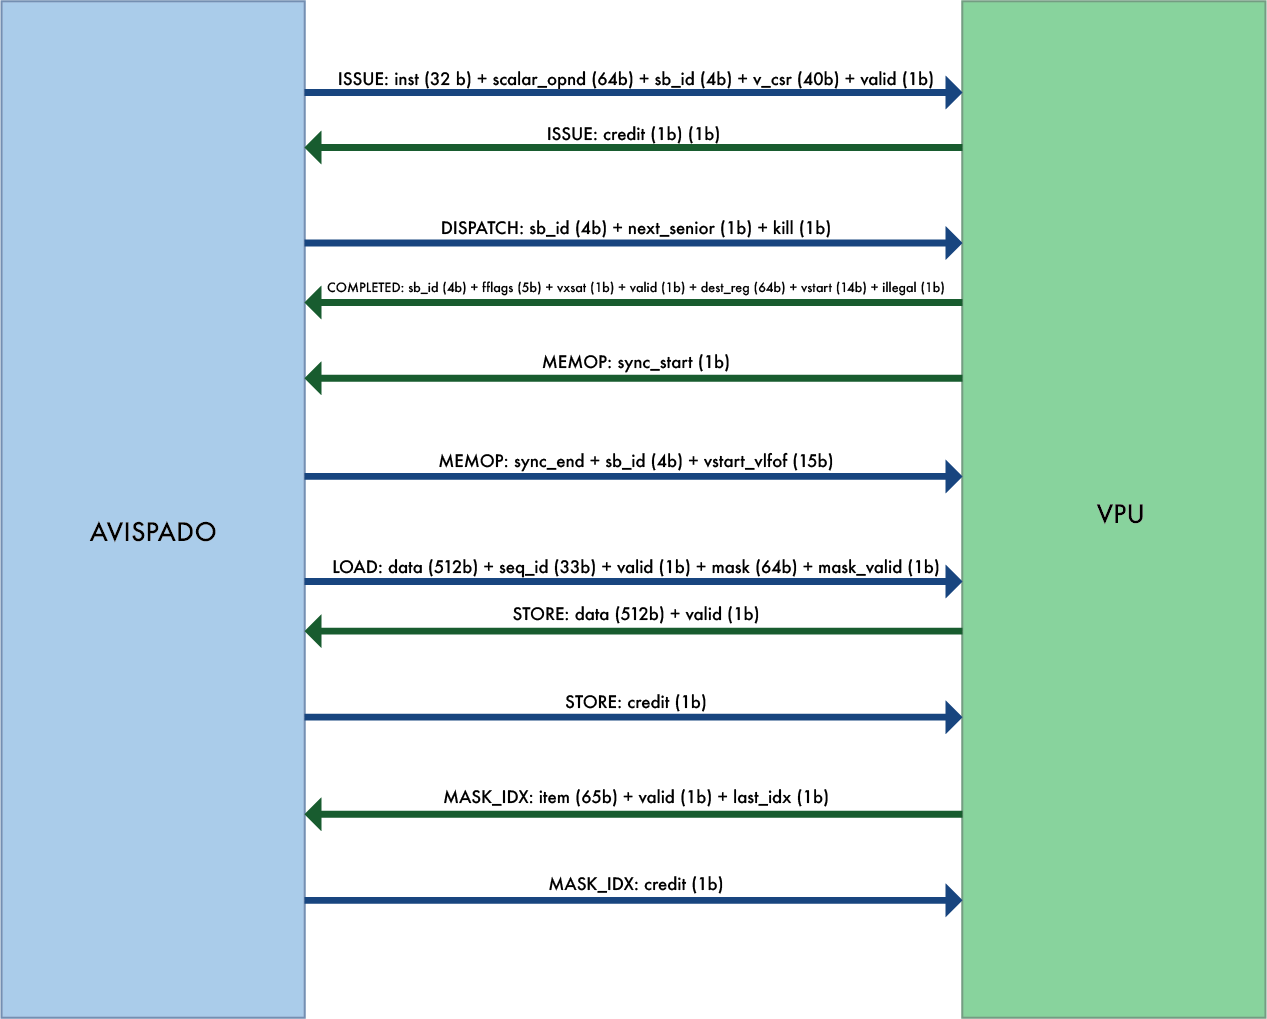
\includegraphics[scale = 0.6]{Chapter_1/img/avi-vpu.png}
    \caption{Avispado-VPU interface}
    \label{avi-vpu}
\end{figure}


The instructions are issued with a credit system, whose number corresponds to the depth of the issue queue of the VPU.



\subsection{The VPU}
In Figure \ref{VPU} it is possible to find a simplified scheme of the implemented VPU.

\begin{figure}[H]
    \centering
    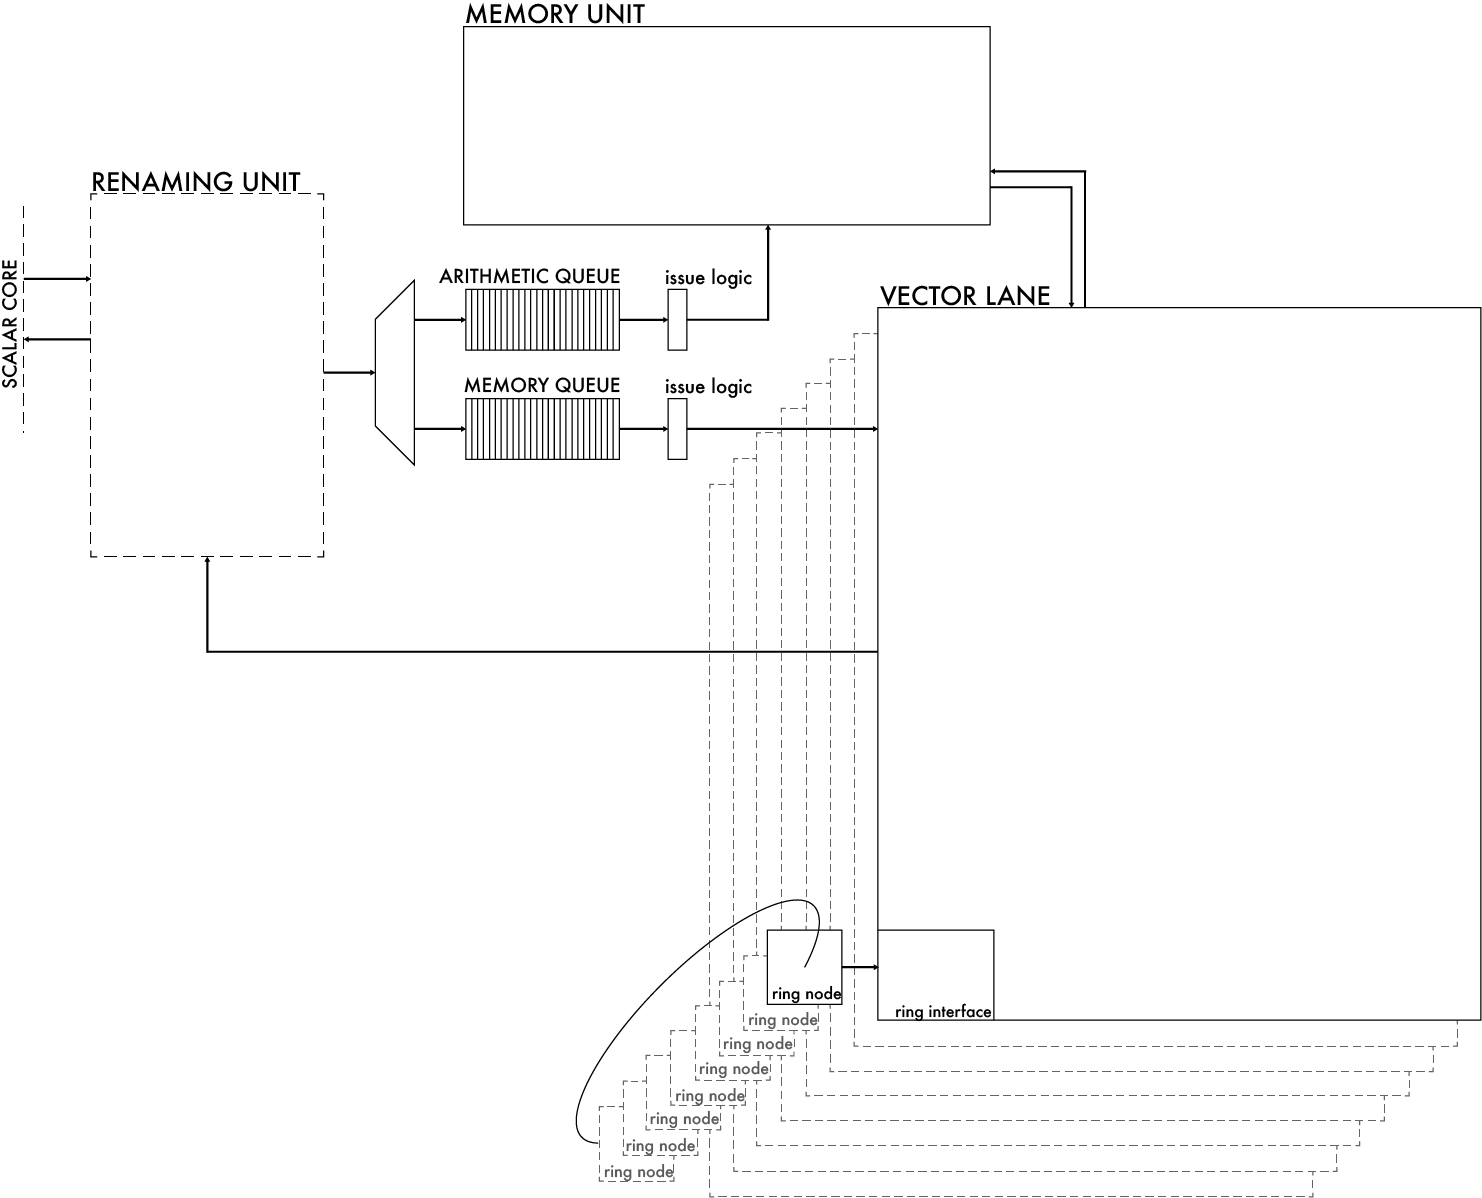
\includegraphics[scale = 0.5]{Chapter_1/img/VPU.png}
    \caption{EPI project's VPU}
    \label{VPU}
\end{figure}
It is important to notice that the VPU implemented is a decoupled architecture, this means that two operations can be executed at once only in case they are not both memory operations nor arithmetic ones.


The main elements composing the VPU are:
\begin{itemize}
    \item \textbf{Renaming Unit}: the scope of this unit is to remove false dependencies due to the naming of the registers. This is possible because of the virtual memory. The processor only uses logical registers, which in this component they are mapped to physical registers using the Free Register List (FRL).
    Write-to-write dependencies are removed if possible, in order to avoid Data Hazards.
 
    \item \textbf{Queues}: the VPU is a decoupled vector architecture, this means that the arithmetic instructions and the memory instructions are buffered in different queues.
    In Figure \ref{VPU} it is possible to see how the two queues are independent in the issue stage.
    The vector lane is capable of performing only one arithmetic instruction at time, so the issue queue must wait until the previous instruction finishes its execution, but simultaneously a memory instruction can be performed.
    The whole issue stage is composed by the queue and the issue logic. The number of entries in the issue queues is parameterized.
    
    \item \textbf{Memory Units}: as mentioned before, the only instructions that can access memory are the load and the store operations. There are different units working on memory instructions: The \emph{load management unit}, the \emph{store management unit} and the \emph{index and mask unit}. As the name suggest their core task is respectively to load operations, to store operations and to mask the operations and provide the indexes.
    The possible addressing modes are strided or indexed.
    
    \item \textbf{Vector Lane}: the Vector Lane is the core of the VPU. It is composed by different vector processing lanes. This is a very common technique that allows to improve performance and scalability.
    In an ideal multi-lane vector architecture all the lanes are working simultaneously and thus efficiently, with the cost of more hardware to control the synchronization.
    
    One of the most important submodules of the Vector Lane is the Vector Register File (VRF). This is designed with only one read/write port, this because it is important to limit the area usage, and so to increase the operating frequency. It is necessary to have a buffer in order to avoid streaming problems and bubbles inside the pipe.
    
    This solution implies the existence of some cost in terms of latency, due to the starting of a new instruction.
    Inside the Vector Lane the Write-Back Buffer (WB) and the Load Buffer (LB) are important as well. Those buffers store the data until the VRF line is complete.
    There is also the Store Buffer (SB) which holds the data read from the register file and then sends it to the Store Unit. 
    Eventually when an instruction is completed the physical register are freed. 
    
    The VPU can be configured with different numbers of lanes from 1 up to 8, the default value is 8.
    
    \item \textbf{Lane Interconnection}: due to the range of the Lanes, which can be any value between 1 and 8, it is important to have a system capable of synchronizing all of them. There are also some operations which require to use multiple lanes at once to perform the execution, so an unidirectional ring intercommunication is implemented between the lanes.
\end{itemize}

It is also important to point out how the memory is organized in order to understand how some operations work.

The vectors are distributed into the different lanes. Indeed it is possible to say the Vector are sliced into the lanes, this means that an efficient organization is needed in order to understand where to put the right data.


According to the RISC-V V-extension, vector elements can have different sizes. The parameter that describes the size of an element is the SEW (Standard Element Width). This is determined by the CSR (Control and Status Register) named vsew. The maximum supported SEW into the EPI project is 64 bit. Also the maximum VLEN is equal to 16384 bit, so 2kB.

The number of elements a vector registers holds is given by VLEN/SEW, according to the Table \ref{sew-el}:


\begin{table}[H]
    \centering
    \begin{tabular}{|l|l|}
    \hline
        \rowcolor[HTML]{C0C0C0} 
        SEW & ELEMENTS \\ \hline
        64  & 256      \\ \hline
        32  & 512      \\ \hline
        16  & 1024     \\ \hline
        8   & 2048     \\ \hline
    \end{tabular}
    %\caption{Caption}
    \label{sew-el}
\end{table}

In Figure \ref{vrf-64} it is possible to see the structure used for SEW = 64 bit as examples.
\begin{figure}[H]
    \centering
    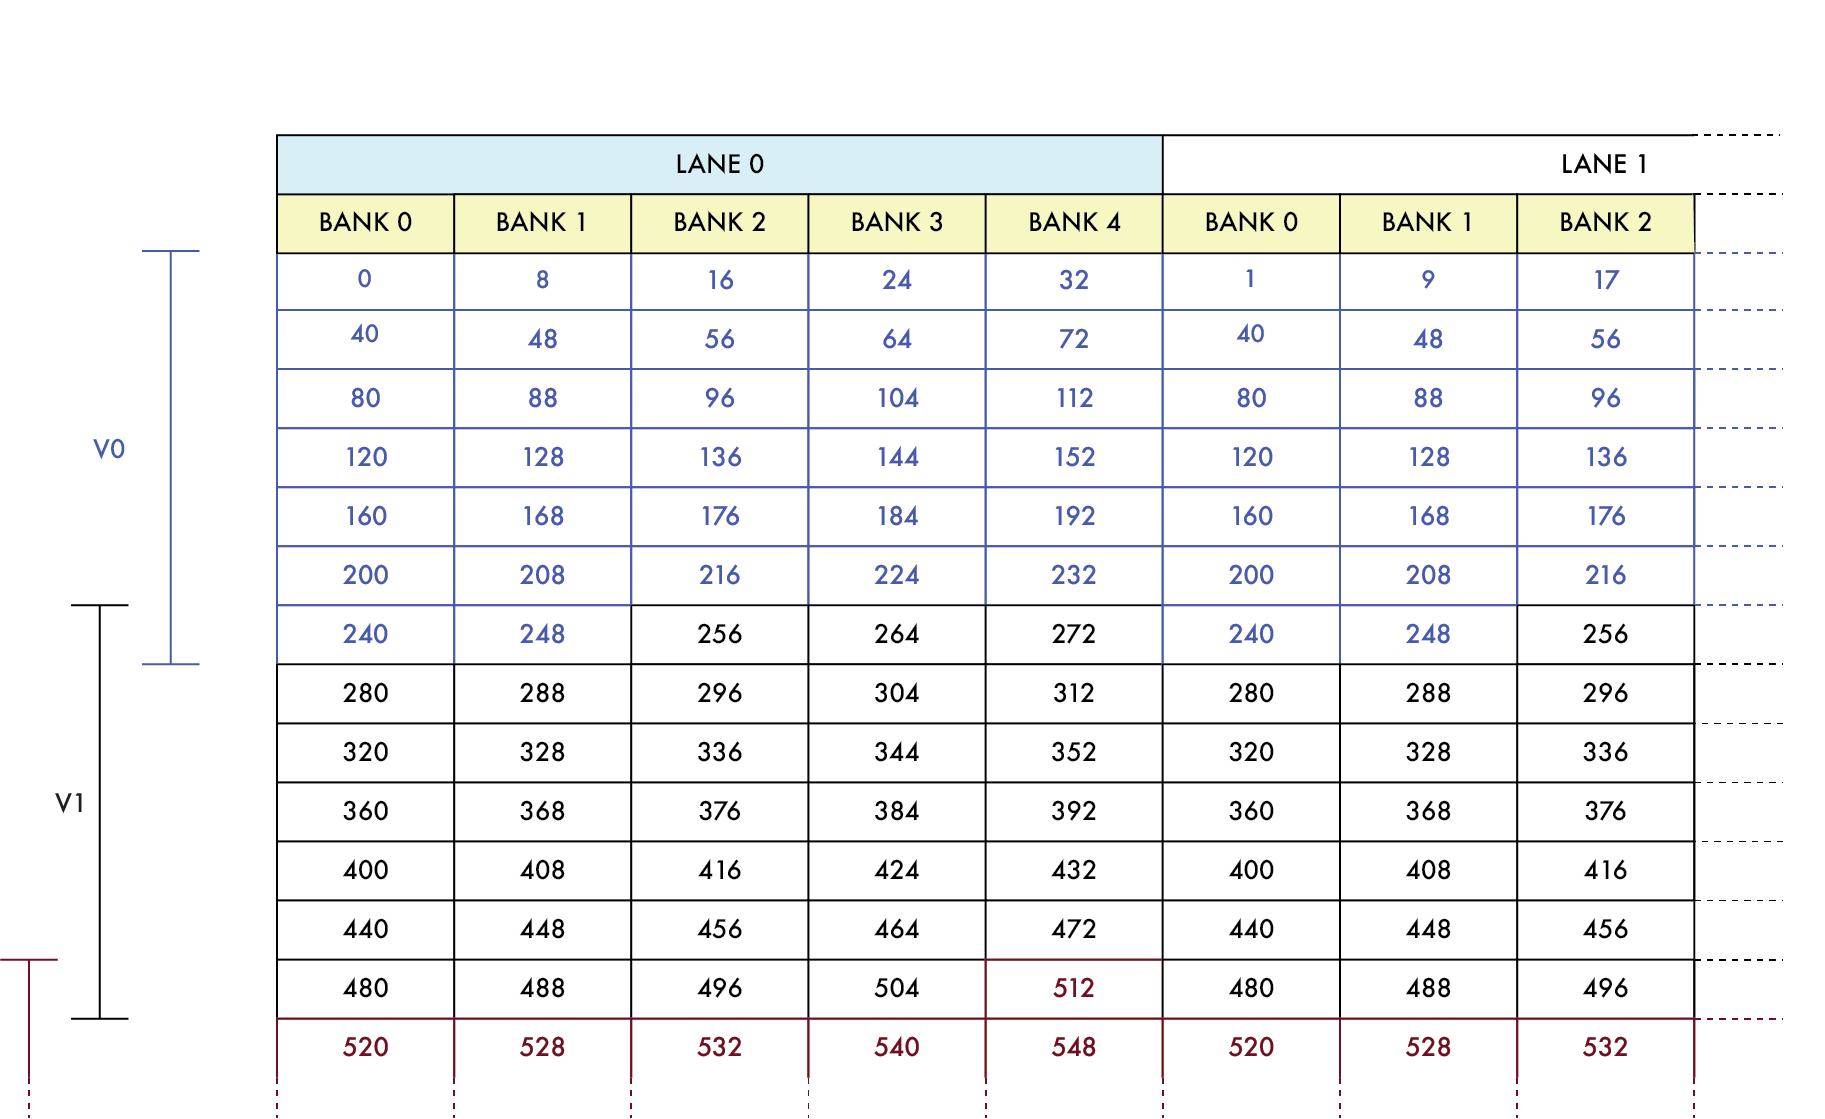
\includegraphics[scale = 0.45]{Chapter_1/img/vrf-64.png}
    \caption{VRF with SEW = 64}
    \label{vrf-64}
\end{figure}

Notice that the sub-banks are more than 1 only when the SEW is not 64. \\

In Figure \ref{vrf-32} it is possible to identify the sub-banks as subdivision of a bank when SEW is not 64.
\begin{figure}[H]
    \centering
    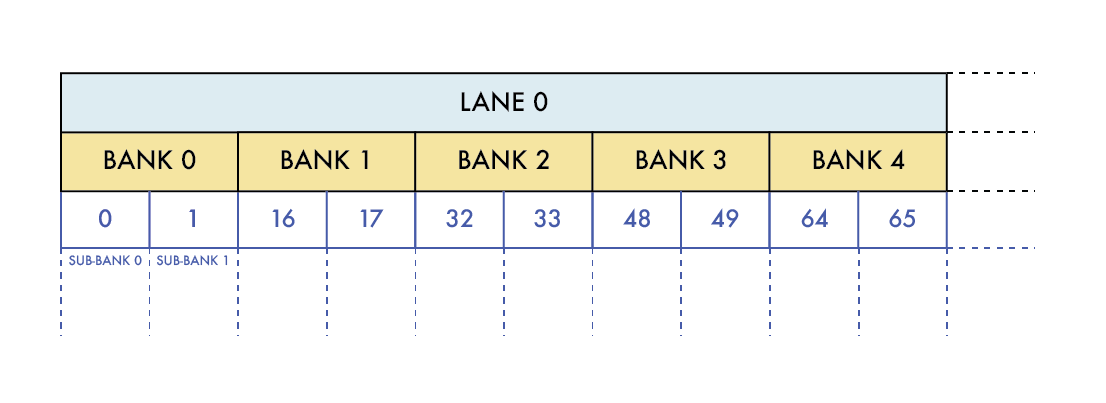
\includegraphics[scale = 0.7]{Chapter_1/img/vrf-32.png}
    \caption{VRF with SEW = 32}
    \label{vrf-32}
\end{figure}

Let's focus now on the submodules on which the work of this thesis was done.




\subsection{The UVM}
As mentioned before, the UVM is the solution to the standardization problem of the verification. In fact, it is a transaction-level methodology (TLM) designed for testbench development. It is a class library that facilitates writing configurable and reusable code \cite{verification-book-2018}.

The testbenches created are designed to be reusable, as a result less code and more production is achieved.

This is mainly obtained with the polymorphism. It means an object can be used to define a reusable class. Operating with this technique an object can be used as a super-class and other sub-classes can be created.

It works following an hierarchy method, and every component can only operate with the components above it. In this way multiple subcomponents can be instantiated.

\subsubsection{Generic UVM}
In Figure \ref{gen-uvm} it is possible to see an example of a standard UVM.

\begin{figure}[H]
    \centering
    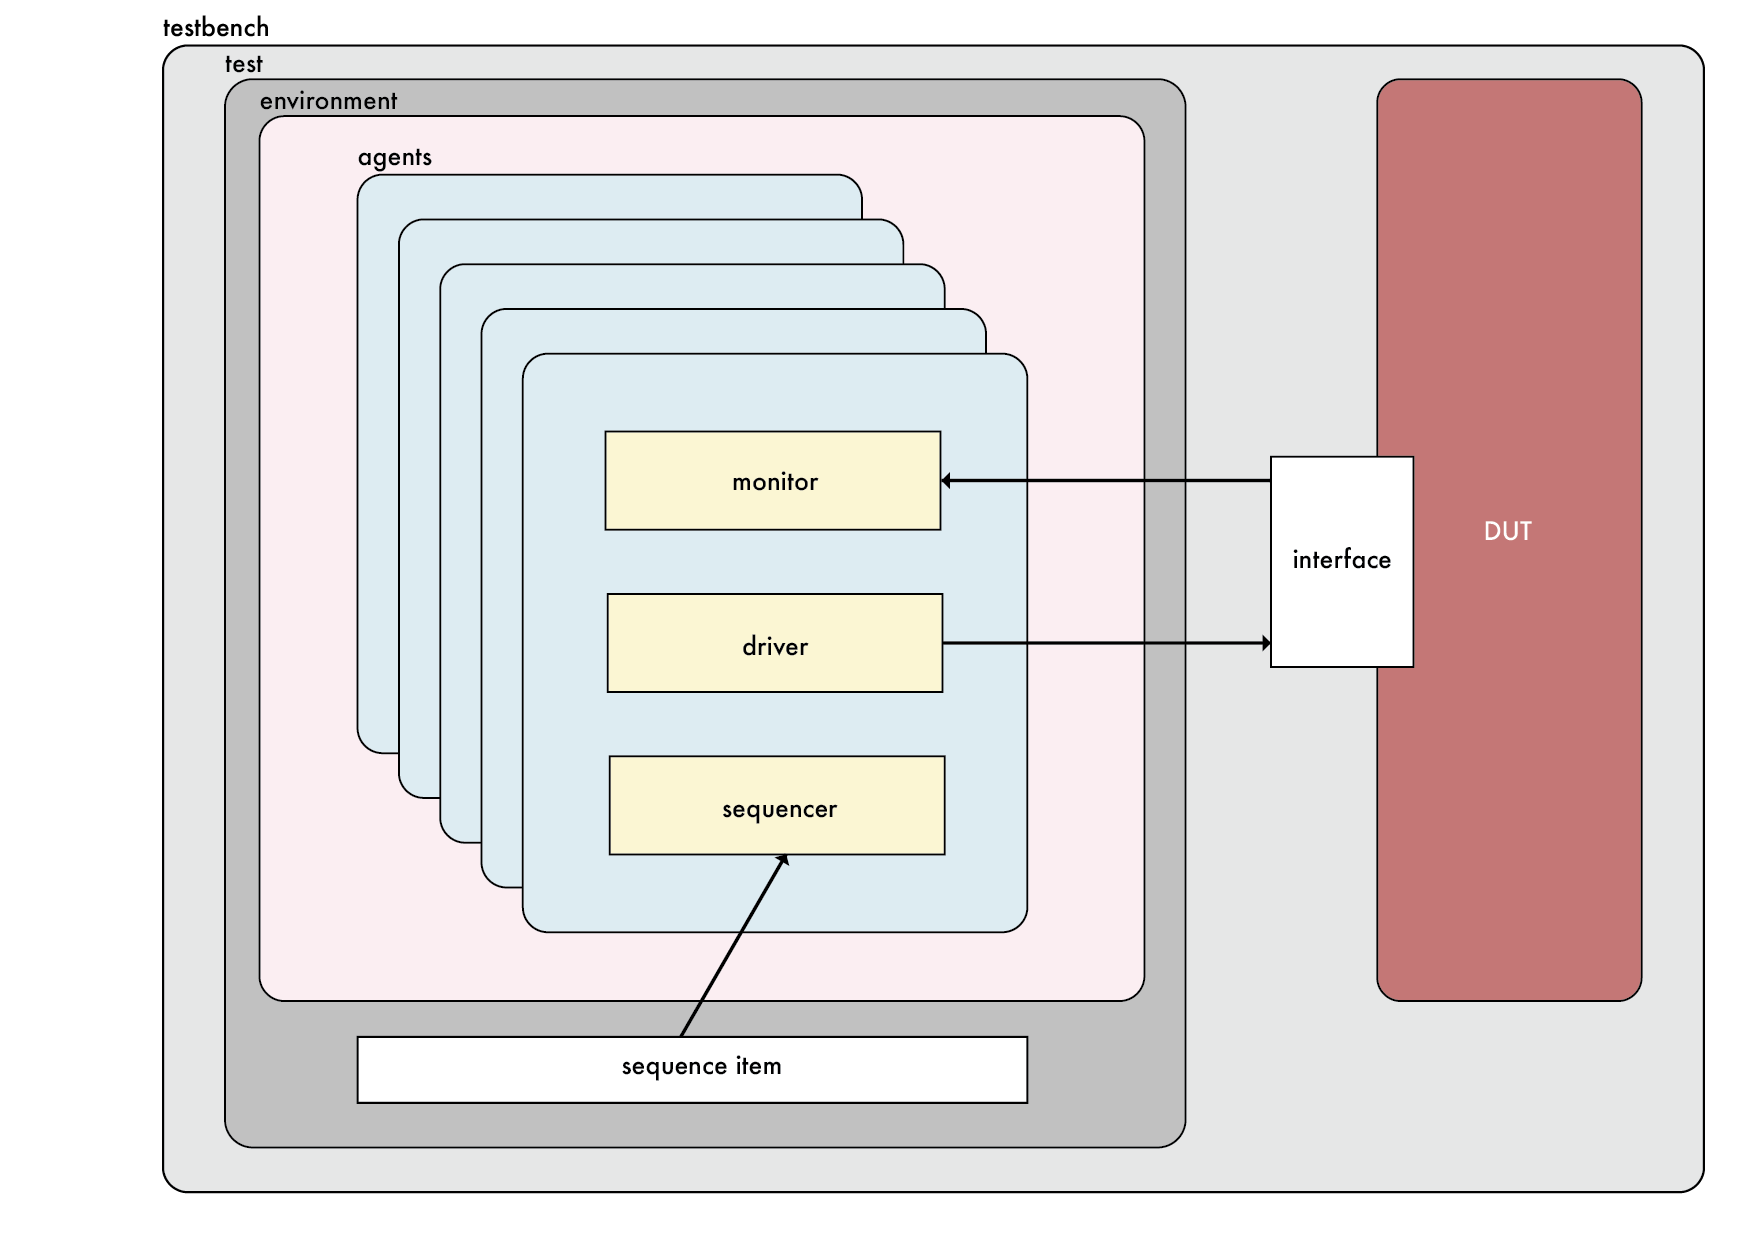
\includegraphics[scale = 0.4]{Chapter_1/img/general-uvm.png}
    \caption{A generic UVM}
    \label{gen-uvm}
\end{figure}

Let's proceed analyzing some elements of a standard UVM and its implementations in the EPI project.

\begin{itemize}
    \item \textbf{Testbench}: typically, it instantiates the DUT (Design Under Test) and the UVM Test Class. Also it is responsible to configure the connections between them.
    There are different ways to communicate into an UVM and in this module is possible to choose them.
    It is also important to say that the Testbench instantiates the Test dynamically at run-time, enabling to compile it once and run many Tests.
    
    \item \textbf{Test}: this is the top-level component into an UVM testbench.
    Typically a base test class is defined to instantiate the top-level environment and then it is extended to the specific case.
    
    \item \textbf{Environment}: it is a component that defines the environment of a test. It aims to define all the agents and the scoreboards. 
    The top-level environment instantiates and configures the reusable verification IP and defines its default configurations based on the application of the test.
    
    Typically there is a different environment for each interface of the DUT.
    
    \item \textbf{Sequence Item}: it is the fundamental lowest denominator object in the UVM hierarchy. It can also be defined as a transaction and it is the smallest data transfer that can exist in a UVM. It can include variables and constraints.
    
    \item \textbf{Sequence}: it is generated by the environment using the sequence item. It is an ordered collection of transactions.
    Mostly it can impose some constraint to the variables generated into the sequence item.
    
    \item \textbf{Agent}: it is one of the most important components of the UVM. It groups together all the components that are dealing with the DUT and so a specific DUT interface.
    Normally there is a different agent for every interface or DUT. This allows specific sequencers for specific stimulus.
    It can also be active or passive depending on its action on the DUT: if it sends signals to stimulate the DUT it is considered active, and otherwise passive.
    
    It contains:
    \begin{itemize}
        \item \textbf{Driver}: it is the component responsible for the communication between the UVM and the DUT at pinlevel. It receives the sequences from the sequencer and then converts them into signals, following the interface protocol.
        This action is observed by another component, the (command) monitor.
        
        It can be turned off when the agent is defined as passive. In this way there is no other component sending signals to the DUT.

        
         \item \textbf{Sequencer}: it controls the requests and the responses between the driver and the sequence item. So it is a controller.
         
        \item \textbf{Monitor}: it observes the outputs of the DUT at pinlevel. Then transforms those signals into transactions for the analysis.
        On a larger stage, those transactions are very likely then compared with the expected outputs. This is normally done in the scoreboard.
        It can perform internally also some processing.
        The signals the monitor is observing could be monitored into the driver, but this would mean violating the modularity choices for the UVM.

        
    \end{itemize}
    
    \item \textbf{Scoreboard}: it is a checker for the outputs of the DUT. It compares the transactions obtained by the monitors against a predicted result.
    There are different ways to generate a predicted result and so a scoreboard, it often uses a C/C++ model, but it is possible to use also other languages as well.
    
\end{itemize}


It is important to point the UVM works in different phases.
It is possible to macro-divide the process in 3 phases: the \textit{build phase}: here the components are constructed from the top, in this phase an important sub-phase is present, the \textit{connect sub-phase}: here all the components are connected upwards; the \textit{run phase}: in this phase the simulation is ran, and finally the \textit{cleanup phase}: here all the results are checked and reported.

In Figure \ref{phases-uvm} it is illustrated a simple scheme representing all the phases.


\begin{figure}[H]
    \centering
    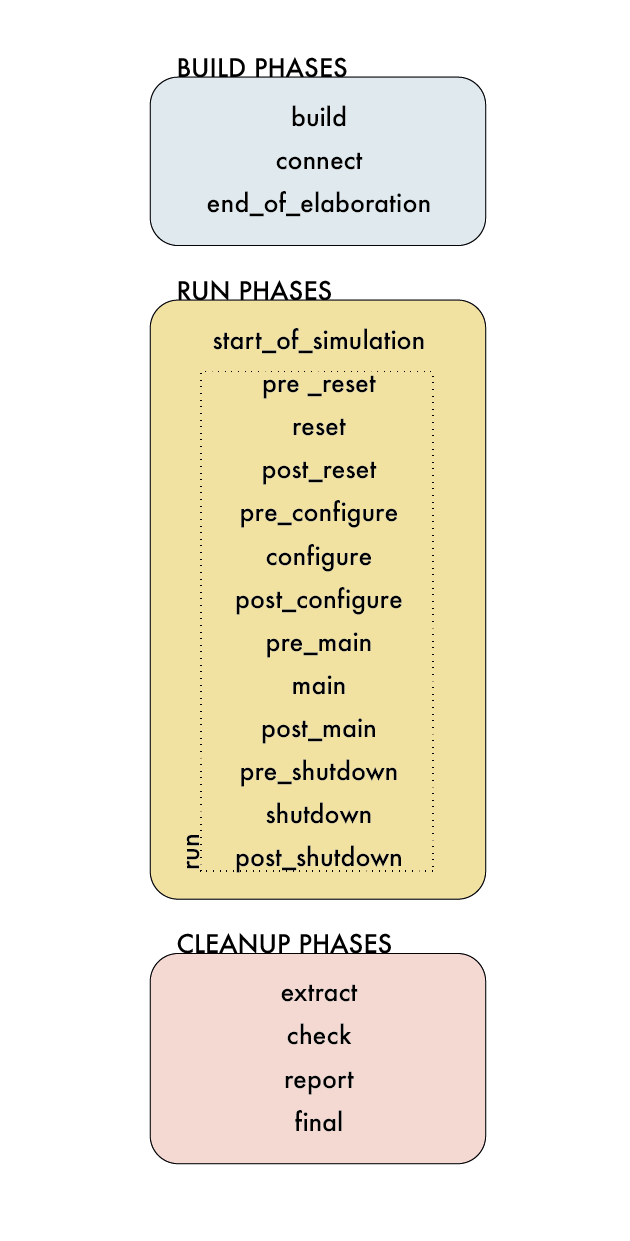
\includegraphics[scale = 0.6]{Chapter_1/img/phases-uvm.png}
    \caption{UVM phases}
    \label{phases-uvm}
\end{figure}


In the EPI project two different UVM structures were implemented. One to test all the VPU (and its interface with the scalar core) and another one to test the submodules. This approach was chosen because it is not always possible to test all the corner cases with an UVM testing the whole VPU.

Let's proceed with a brief analysis of those two structures.

\subsubsection{Main UVM}
The main UVM is interfaced with Avispado and it is composed following the standard structure. It was mainly used to support the use of a scoreboard (Spike) and then to implement then some checkers and some coverage controls.

The majority of the automatic tests are made with this structure, and they are scripted to run all the night and to produce a valid dataset to then find and fix the bugs. Those tests are created using random RISC-V vector instructions, with some constraints that allow the tests to be valid.

Using a simulator for Avispado as input, the driver is a little bit different from a standard one. Indeed, the input are not controlled at pinlevel but vector instructions are sent to the core, which will then produce a correct input for the VPU.

Those instructions are ultimately compared with with the scoreboard and a result is produced.

\subsubsection{Submodules UVM}

Another structure was necessary due to the different interface, and so to different drivers. It is not always trivial to create a driver for a submodule, because the handshake processes can be very complex, thus it would be possible to introduce some error in the verification structure.


As an UVM structure is useful when driving an monitoring all the signals of a module, this technique was used for the Load Management Unit but not for the Load Buffer. This because the handshake process for the Load Buffer is complex, and so would have been the UVM, with the possibility to introduce some errors.
The structure of the LMU's UVM is represented in figure \ref{sub-uvm}.

\begin{figure}[H]
    \centering
    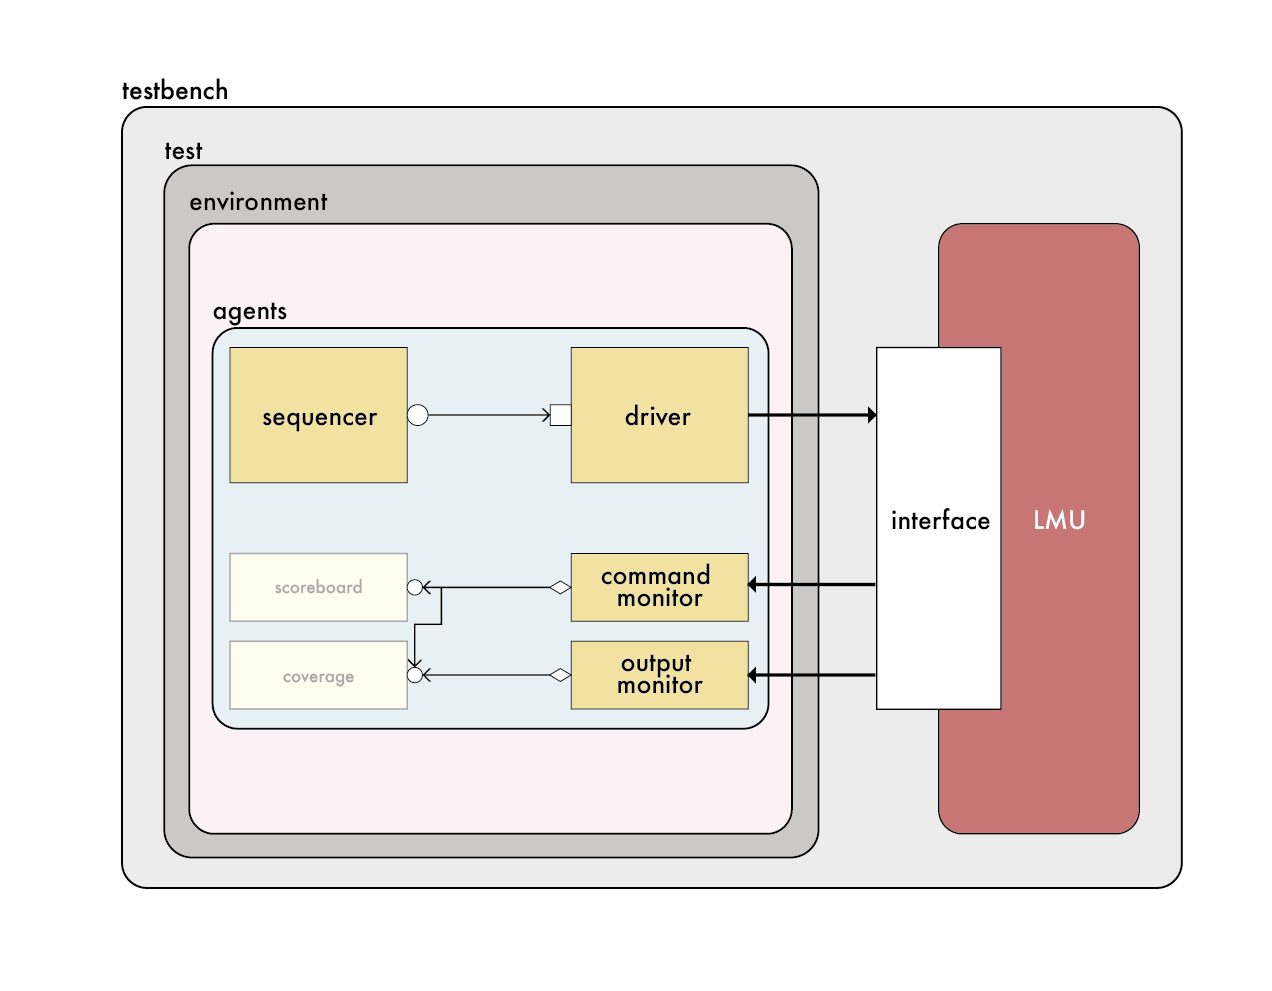
\includegraphics[scale = 0.7]{Chapter_1/img/sub-uvm.png}
    \caption{A small UVM for the submodules}
    \label{sub-uvm}
\end{figure}

It is possible to observe the scoreboard and the coverage are disabled in this application. In reality a scoreboard was implemented for each of them, but was handles with a different methodology discussed later on the next Chapter.